\documentclass[11pt,a4paper]{article}

\usepackage[margin=2.5cm]{geometry}
\usepackage{booktabs}
\usepackage{float}
\usepackage{tabularx}
\usepackage{xltabular}
\usepackage{array}
\usepackage{enumitem}
\usepackage{totcount}
\usepackage{fancyhdr}
\usepackage{lastpage}
\usepackage{needspace}
\usepackage{bytefield}
\usepackage{tikz}
\usetikzlibrary{arrows.meta,positioning,fit,calc,decorations.pathreplacing}
\usepackage[hidelinks]{hyperref}
\setlength{\emergencystretch}{1.5em}

% Section numbers in the same style as the ConOps: 1.0, 1.1.
\renewcommand{\thesection}{\arabic{section}.0}
\renewcommand{\thesubsection}{\arabic{section}.\arabic{subsection}}

% Controlled-document header on every page.
\newcommand{\docref}{Reference TBD}
\newcommand{\docrev}{Issue 1, Rev.~0 --- DRAFT}
\pagestyle{fancy}
\fancyhf{}
\lhead{\footnotesize Fail-Safe In-Orbit Reprogramming of a Spacecraft Controller --- Interface Design}
\lfoot{\small \docref}
\cfoot{\small \docrev}
\rfoot{\small Page \thepage\ of \pageref{LastPage}}

% Open items. TBD = not known. TBR = proposal awaiting the author's
% acceptance. Listed in App. C; totals counted, not typed.
\newtotcounter{tbd}
\newtotcounter{tbr}
\newcommand{\tbditem}[2]{\refstepcounter{tbd}\label{tbd:#1}\item[TBD-\thetbd] #2}
\newcommand{\tbritem}[2]{\refstepcounter{tbr}\label{tbr:#1}\item[TBR-\thetbr] #2}
\newcommand{\tbd}[1]{\mbox{\textbf{[\hyperref[tbd:#1]{TBD-\ref*{tbd:#1}}]}}}
\newcommand{\tbr}[1]{\mbox{\textbf{[\hyperref[tbr:#1]{TBR-\ref*{tbr:#1}}]}}}

\setlist[description]{style=multiline,leftmargin=2cm,nosep,font=\normalfont\bfseries}
\setlist[itemize]{nosep}

\begin{document}

\thispagestyle{fancy}
\begin{center}
{\LARGE\bfseries Fail-Safe In-Orbit Reprogramming\\[0.2em] of a Spacecraft Controller\par}
\vspace{0.4em}
{\Large Interface Design Description\par}
\vspace{1em}
\begin{tabular}{@{}ll@{}}
Reference & TBD \tbd{ref} \\
Issue / revision & Issue 1, Revision 0 --- DRAFT \\
Date & 12 October 2026 \\
Author & Andrew Toma \\
Open items & \total{tbd} TBD, \total{tbr} TBR (App.~C) \\
\end{tabular}
\end{center}

\subsection*{Document change record}
\begin{tabular}{@{}llll@{}}
\toprule
Issue & Rev. & Date & Change \\
\midrule
1 & 0 & 2026-10-12 & First draft \\
\bottomrule
\end{tabular}

% ===========================================================================
\section{Purpose and Scope}
This document defines each interface identified in the architecture
[2,~Sec.~7.0]: the format and content of every data element that crosses it,
its communication method and protocol, and the signals between the two
units. It covers the minimum content of an interface design
description [1,~Sec.~1].

% ===========================================================================
\section{Documents}
\noindent [1] NASA, \emph{NASA Software Engineering Handbook}, NASA-HDBK-2203,
Version~D, Topic 5.02 ``IDD -- Interface Design Description''.

\noindent [2] \emph{Fail-Safe In-Orbit Reprogramming of a Spacecraft
Controller --- Software Architecture}, Issue~1, Revision~0, Draft.

\noindent [3] \emph{Fail-Safe In-Orbit Reprogramming of a Spacecraft
Controller --- Software Requirements Specification}, Issue~1, Revision~0,
Draft.

\noindent [4] \emph{Fail-Safe In-Orbit Reprogramming of a Spacecraft
Controller --- Hazard Analysis}, Issue~1, Revision~1, Draft.

\noindent [5] \emph{Fail-Safe In-Orbit Reprogramming of a Spacecraft
Controller --- Concept of Operations}, Issue~1, Revision~1, Draft.

\noindent [6] S.~Josefsson and I.~Liusvaara, \emph{Edwards-Curve Digital
Signature Algorithm (EdDSA)}, RFC~8032, January 2017.

\noindent [7] NIST, \emph{Recommendation for Block Cipher Modes of Operation:
Galois/Counter Mode (GCM) and GMAC}, SP 800-38D, November 2007.

\noindent [8] Arm, \emph{ARM Debug Interface v5 Architecture Specification},
IHI 0031A, 2006.

\noindent [9] STMicroelectronics, \emph{STM32G4 Series Reference Manual},
RM0440 Rev~9.

\noindent [10] STMicroelectronics, \emph{How to Use the USART Protocol in the
Bootloader on STM32 MCUs}, AN3155 Rev~22.

\noindent [11] STMicroelectronics, \emph{Introduction to System Memory Boot
Mode on STM32 MCUs}, AN2606 Rev~70.

\noindent [12] Texas Instruments, \emph{RS-422 and RS-485 Standards Overview
and System Configurations}, SLLA070D, May 2010.

\noindent [13] NASA, \emph{State-of-the-Art Small Spacecraft Technology},
NASA/TP-20260003140, May 2026, Chapter~8 ``Small Spacecraft Avionics''.

\noindent [14] Texas Instruments, \emph{Introduction to the Controller Area
Network (CAN)}, SLOA101B, May 2016.

% ===========================================================================
\section{Overview}
Figure~\ref{fig:context} shows every interface and the signals it uses.
Table~\ref{tab:kinds} gives each interface's type, priority and use, and
whether it is safety-critical [1,~Sec.~1].

\begin{figure}[H]
\centering
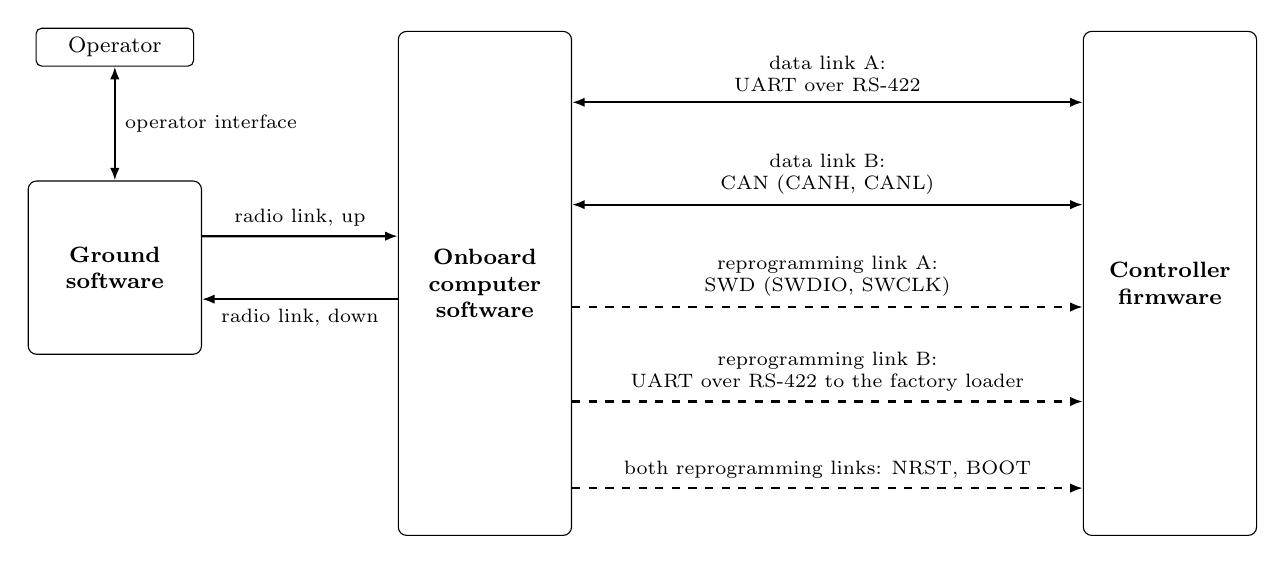
\begin{tikzpicture}[font=\footnotesize,
  blk/.style={draw, rounded corners=3pt, minimum width=2.2cm, minimum height=6.4cm, align=center, font=\footnotesize\bfseries},
  ar/.style={-{Latex[length=1.6mm]}, thick},
  ar2/.style={{Latex[length=1.6mm]}-{Latex[length=1.6mm]}, thick},
  lab/.style={font=\scriptsize, align=center}]
\node[draw, rounded corners=2pt, minimum width=2.0cm] (op) at (0,3.0) {Operator};
\node[blk, minimum height=2.2cm] (g) at (0,0.2) {Ground\\software};
\node[blk] (o) at (4.7,0) {Onboard\\computer\\software};
\node[blk] (c) at (13.4,0) {Controller\\firmware};
\draw[ar2] (op) -- node[right, lab]{operator interface} (g);
\draw[ar] ($(g.east)+(0,0.4)$) -- node[above, lab]{radio link, up} ($(o.west)+(0,0.6)$);
\draw[ar] ($(o.west)+(0,-0.2)$) -- node[below, lab]{radio link, down} ($(g.east)+(0,-0.4)$);
\draw[ar2] ($(o.east)+(0,2.3)$) -- node[above, lab]{data link A:\\UART over RS-422} ($(c.west)+(0,2.3)$);
\draw[ar2] ($(o.east)+(0,1.0)$) -- node[above, lab]{data link B:\\CAN (CANH, CANL)} ($(c.west)+(0,1.0)$);
\draw[ar, dashed] ($(o.east)+(0,-0.3)$) -- node[above, lab]{reprogramming link A:\\SWD (SWDIO, SWCLK)} ($(c.west)+(0,-0.3)$);
\draw[ar, dashed] ($(o.east)+(0,-1.5)$) -- node[above, lab]{reprogramming link B:\\UART over RS-422 to the factory loader} ($(c.west)+(0,-1.5)$);
\draw[ar, dashed] ($(o.east)+(0,-2.6)$) -- node[above, lab]{both reprogramming links: NRST, BOOT} ($(c.west)+(0,-2.6)$);
\end{tikzpicture}
\caption{The interfaces and their signals. Solid: used in operation. Dashed:
used only to restore or reload the controller.}
\label{fig:context}
\end{figure}

\begin{table}[H]
\centering
{\small\begin{tabularx}{\textwidth}{@{}l>{\raggedright\arraybackslash}Xlll@{}}
\toprule
Interface & Type & Priority & Used & Safety-critical \\
\midrule
Operator interface & Commands in, state out & ONLY & ALWAYS & YES \\
Radio link & Data transfer, encrypted and signed & ONLY & AT CONTACTS & YES \\
Data link A & Data transfer & PRIMARY & ALWAYS & YES \\
Data link B & Data transfer & BACKUP & ALWAYS & YES \\
Reprogramming link A & Memory load & PRIMARY & RESTORE & YES \\
Reprogramming link B & Memory load & BACKUP & RESTORE & YES \\
\bottomrule
\end{tabularx}}
\caption{Interface types \tbr{priority}.}
\label{tab:kinds}
\end{table}

\vspace{-0.6em}
\noindent{\small\textbf{Legend.} Priority: ONLY, the one interface for its
traffic; PRIMARY, used first; BACKUP, used when the primary one is lost.
Used: ALWAYS, whenever the System runs; AT CONTACTS, during contact windows;
RESTORE, during a restore or a reload through the reprogramming link.}

% ===========================================================================
\section{Message Layer}
\label{sec:frame}
Every command, answer and report travels in the same frame on the radio link
and on both data links (Figure~\ref{fig:frame}). Multi-byte fields are
little-endian. The check value is a CRC-32 of every byte before it. The receiver computes it again; a different result means the
frame was damaged on the way. The polynomial is 0x4C11DB7, the one the
controller's processor computes in hardware. It stands for
$x^{32}+x^{26}+x^{23}+x^{22}+x^{16}+x^{12}+x^{11}+x^{10}+x^{8}+x^{7}+x^{5}+x^{4}+x^{2}+x+1$
[9,~Sec.~16.2, p.~454]: each 1 bit marks a power of $x$, and the top term
$x^{32}$ is left out of the hexadecimal. The calculation starts from
0xFFFFFFFF, takes each byte least significant bit first, and inverts the
result. A receiver drops a frame whose check value or version it does not
accept.

\begin{figure}[H]
\centering
\begin{bytefield}[bitwidth=0.42cm]{32}
\bitbox[]{8}{\scriptsize byte 0} & \bitbox[]{8}{\scriptsize byte 1} & \bitbox[]{8}{\scriptsize byte 2} & \bitbox[]{8}{\scriptsize byte 3} \\
\bitbox{16}{Sync} & \bitbox{8}{Version} & \bitbox{8}{Type} \\
\bitbox{8}{Destination} & \bitbox{8}{Flags} & \bitbox{16}{Length} \\
\wordbox{1}{Sequence number} \\
\wordbox{1}{Expiry} \\
\wordbox[lrt]{1}{Payload: Length bytes} \\
\skippedwords \\
\wordbox[lrb]{1}{} \\
\wordbox{1}{Check value} \\
\end{bytefield}
\caption{The frame. Each row is four bytes. The header is the first 16
bytes.}
\label{fig:frame}
\end{figure}

{\small\noindent\begin{tabularx}{\textwidth}{@{}lc>{\raggedright\arraybackslash}p{3.6cm}>{\raggedright\arraybackslash}X@{}}
\toprule
Field & Bytes & Values & Meaning \\
\midrule
Sync & 2 & 0xA5, 0x5A & Start of a frame \\
Version & 1 & 0x01 & Frame format version \\
Type & 1 & 0x01 command, 0x02 answer, 0x03 report & What the payload holds \\
Destination & 1 & 0x01 onboard computer, 0x02 controller, 0x03 ground & Who acts on the frame \\
Flags & 1 & bit 0 & Set when the onboard computer releases a scheduled command; other bits 0 \\
Length & 2 & 0 to 1024 & Payload length in bytes \\
Sequence number & 4 & 1 to $2^{32}-1$ & One higher than the sender's last frame [3,~REQ-065] \\
Expiry & 4 & seconds of ground time & After it, the command is refused [3,~REQ-066, REQ-133]; 0 in answers and reports \\
Payload & Length & & The command, answer or report \\
Check value & 4 & CRC-32 & Detects damage to the frame [3,~REQ-107] \\
\bottomrule
\end{tabularx}}

\subsection{Radio Envelope}
On the radio link each frame travels inside an envelope
(Figure~\ref{fig:envelope}). The frame is signed twice with Ed25519, an
elliptic-curve digital signature scheme, each signature 64 bytes
[6,~Sec.~1]. The frame and both signatures are then
encrypted with AES-256 in Galois/Counter Mode, with a 12-byte nonce and a
16-byte tag [7,~Secs.~5.2.1.1--5.2.1.2, pp.~8--9]. The link
encryptor builds the envelope. The onboard computer opens it, checks both
signatures, and acts only when all three checks pass [3,~REQ-127 to
REQ-129].

\begin{figure}[H]
\centering
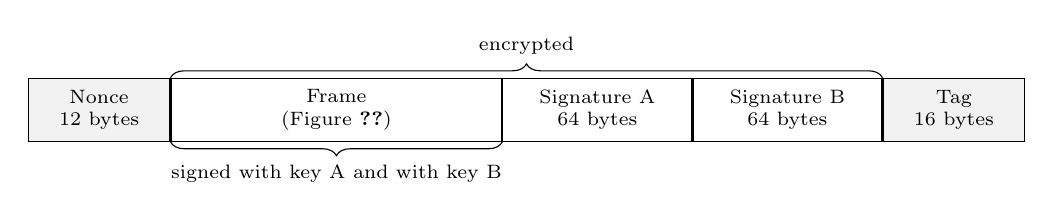
\begin{tikzpicture}[font=\scriptsize,
  seg/.style={draw, minimum height=0.8cm, align=center, inner sep=1pt}]
\node[seg, minimum width=1.8cm, fill=black!5] (n) at (0,0) {Nonce\\12 bytes};
\node[seg, minimum width=4.2cm, right=0pt of n] (f) {Frame\\(Figure~\ref{fig:frame})};
\node[seg, minimum width=2.4cm, right=0pt of f] (a) {Signature A\\64 bytes};
\node[seg, minimum width=2.4cm, right=0pt of a] (b) {Signature B\\64 bytes};
\node[seg, minimum width=1.8cm, fill=black!5, right=0pt of b] (t) {Tag\\16 bytes};
\draw[decorate, decoration={brace, amplitude=5pt}] (f.north west) -- node[above=5pt]{encrypted} (b.north east);
\draw[decorate, decoration={brace, amplitude=5pt, mirror}] (f.south west) -- node[below=5pt]{signed with key A and with key B} (f.south east);
\end{tikzpicture}
\caption{The radio envelope. The tag proves the encrypted part unchanged and
encrypted with the right key; the signatures prove the frame comes from the
operator.}
\label{fig:envelope}
\end{figure}

\subsection{Answers}
\label{sec:answers}
Every command gets two answers [3,~REQ-033]: RECEIVED when it passes the
checks on arrival, then DONE with its result or REFUSED with a reason
(Figure~\ref{fig:answers}). A command sent again with a sequence number
already run is answered ALREADY DONE and is not run twice [3,~REQ-031]. An
envelope that fails any of its checks is dropped and logged without an
answer, so that a sender without the keys learns nothing [3,~REQ-064]
\tbr{silent}.

\begin{figure}[H]
\centering
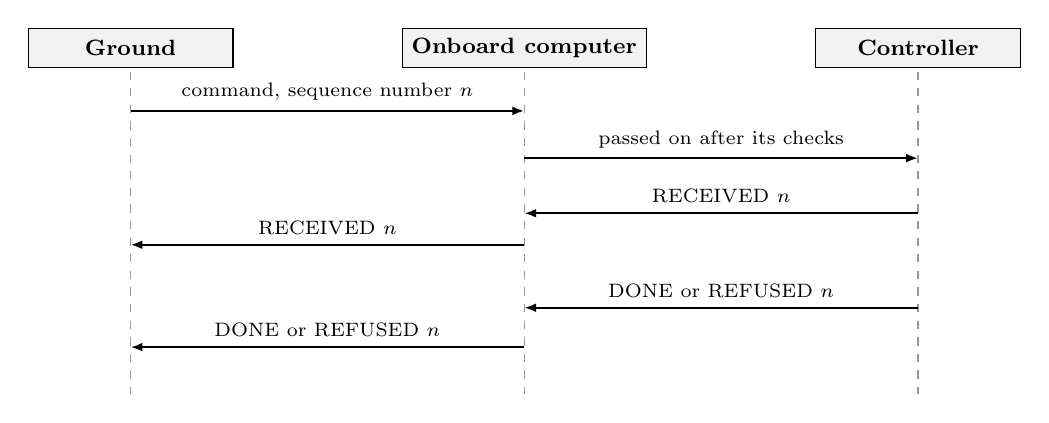
\begin{tikzpicture}[font=\scriptsize,
  head/.style={draw, fill=black!5, minimum width=2.6cm, minimum height=0.5cm, font=\footnotesize\bfseries},
  msg/.style={-{Latex[length=1.5mm]}, thick}]
\node[head] at (0,0) {Ground};
\node[head] at (5,0) {Onboard computer};
\node[head] at (10,0) {Controller};
\foreach \x in {0,5,10} \draw[dashed, black!40] (\x,-0.3) -- (\x,-4.4);
\draw[msg] (0,-0.8) -- node[above]{command, sequence number $n$} (5,-0.8);
\draw[msg] (5,-1.4) -- node[above]{passed on after its checks} (10,-1.4);
\draw[msg] (10,-2.1) -- node[above]{RECEIVED $n$} (5,-2.1);
\draw[msg] (5,-2.5) -- node[above]{RECEIVED $n$} (0,-2.5);
\draw[msg] (10,-3.3) -- node[above]{DONE or REFUSED $n$} (5,-3.3);
\draw[msg] (5,-3.8) -- node[above]{DONE or REFUSED $n$} (0,-3.8);
\end{tikzpicture}
\caption{A command to the controller and its two answers. DONE carries the
result, REFUSED the reason. A command to the onboard computer is answered by
the onboard computer.}
\label{fig:answers}
\end{figure}

\noindent An answer's payload is six bytes: the sequence number answered (4 bytes); the
kind (1 byte): 0x01 RECEIVED, 0x02 DONE, 0x03 REFUSED, 0x04 ALREADY DONE; and
a code (1 byte): for DONE, 0x00 on success; for REFUSED, the reason below.
The ground and the onboard software share this list [3,~REQ-100].

{\small\noindent\begin{tabularx}{\textwidth}{@{}l>{\raggedright\arraybackslash}Xl@{}}
\toprule
Code & Reason & Requirement \\
\midrule
0x01 & Dangerous command without a valid arming command & REQ-029, REQ-112 \\
0x02 & Arming command expired & REQ-030 \\
0x03 & Command past its expiry & REQ-066, REQ-133 \\
0x04 & Old command sent again & REQ-065 \\
0x05 & Not allowed in the current mode & REQ-027 \\
0x06 & Impossible values, or an unknown command & REQ-028 \\
0x07 & No new firmware during a trial & REQ-050 \\
0x08 & Image damaged & REQ-005, REQ-044 \\
0x09 & Image not from the operator & REQ-006, REQ-043 \\
0x0A & Image older than the minimum version & REQ-045 \\
0x0B & Image built for another controller & REQ-046 \\
0x0C & The controller's clock disagrees with the scheduled time & REQ-134 \\
0x0D & A dangerous command cannot be scheduled & \tbr{sched} \\
\bottomrule
\end{tabularx}}

% ===========================================================================
\section{Commands, Reports and Firmware Images}

\subsection{Commands}
\label{sec:commands}
A command's payload is its one-byte identifier followed by its fields.
Identifiers 0x01 to 0x1F are commands to the onboard computer, 0x20 to 0x3F
commands to the controller.

{\footnotesize
\begin{xltabular}{\textwidth}{@{}l>{\raggedright\arraybackslash}p{3.3cm}>{\raggedright\arraybackslash}X>{\raggedright\arraybackslash}p{1.9cm}cl@{}}
\toprule
ID & Command & Fields (bytes) & Modes & Dangerous & Requirement \\
\midrule
\endhead
0x01 & UPLOAD BEGIN & image number (2), image length (4) & ANY & NO & REQ-049 \\
0x02 & UPLOAD CHUNK & image number (2), offset (4), data (up to 256) & ANY & NO & REQ-049 \\
0x03 & UPLOAD END & image number (2) & ANY & NO & REQ-043 to 047 \\
0x04 & UPLOAD CANCEL & image number (2) & ANY & NO & REQ-051 \\
0x05 & DELIVER & image number (2) & OPERATE, FALLBACK & NO & REQ-048, REQ-050 \\
0x06 & SET LIMITS & minimum version (4), controller identity (2) & ANY & YES & REQ-053 \\
0x07 & RESTORE & none & ANY & YES & REQ-055 \\
0x08 & REPROGRAM & image number (2), region (1): bootloader, main firmware or last-resort firmware & ANY & YES & REQ-058, REQ-121 \\
0x09 & SET ONBOARD TIME & ground time (4) & ANY & YES & REQ-073 \\
0x0A & SCHEDULE & run time (4), one complete frame & ANY & NO & REQ-068 \\
0x0B & SEND REPORTS & first report number (4) & ANY & NO & REQ-074 \\
0x0C & REPLACE KEY & which key (1): signing A, signing B or encryption; new key (32) & ANY & YES & REQ-084 to 086 \\
0x0D & ARM & command identifier (1), its sequence number (4) & ANY & NO & REQ-029, REQ-112 \\
0x20 & SWITCH & none & OPERATE, FALLBACK & YES & REQ-021 \\
0x21 & RETURN TO PREVIOUS & none & OPERATE, TRIAL & YES & REQ-113 \\
0x22 & START FAILED & which copy (1) & OPERATE, FALLBACK & YES & REQ-019 \\
0x23 & LEAVE FALLBACK & none & FALLBACK & NO & REQ-117 \\
0x24 & SET CONTROLLER TIME & ground time (4) & OPERATE, TRIAL, FALLBACK & YES & REQ-132 \\
0x25 & GET STATUS & none & OPERATE, TRIAL, FALLBACK & NO & REQ-081 \\
0x40 & EQUIPMENT & set by the controlled equipment & \tbd{equip} & \tbd{equip} & --- \\
\bottomrule
\end{xltabular}}

\vspace{-0.8em}
\noindent{\small\textbf{Legend.} Modes: the controller modes in which the
command is accepted, within those that accept commands [5,~Sec.~3.4]; ANY,
every mode, RECOVERY included. Dangerous: YES, it needs an arming command
first [3,~REQ-029, REQ-112]; NO, it does not \tbr{dangerous}.}

\subsection{Arming}
An ARM command names the one dangerous command it allows, by identifier and
sequence number \tbr{armone}. It allows no other command, and it expires after
\tbd{arm} [3,~REQ-030]. The onboard computer and the controller each check it
[3,~REQ-029, REQ-112].

\subsection{Scheduled Commands}
\label{sec:sched}
SCHEDULE holds a complete frame on the onboard computer until its run time
[3,~REQ-068]. At that time the onboard computer checks the frame again
against its check value [3,~REQ-136] and passes it to the controller with
Flags bit~0 set. The controller runs it only if its own clock agrees with the
run time within \tbd{agree} [3,~REQ-134]. A dangerous command cannot be
scheduled, because no operator is present at run time to arm it \tbr{sched}.

\subsection{Reports}
The controller sends a HEALTH report at \tbd{rate} and an EVENT report as
soon as an event happens [3,~REQ-037]. The onboard computer adds the report
number and its own clock time before storing the report [3,~REQ-070, REQ-071,
REQ-135].

{\footnotesize
\begin{xltabular}{\textwidth}{@{}l>{\raggedright\arraybackslash}Xcl@{}}
\toprule
Report & Field & Bytes & Set by \\
\midrule
\endhead
ALL & report number & 4 & onboard computer \\
ALL & onboard computer clock time & 4 & onboard computer \\
ALL & controller clock time & 4 & controller \\
ALL & report kind: 0x01 HEALTH, 0x02 EVENT & 1 & controller \\
HEALTH & mode: 0x01 OPERATE, 0x02 TRIAL, 0x03 FALLBACK & 1 & controller \\
HEALTH & running firmware: kind (1), version (4) & 5 & controller \\
HEALTH & failed starts of the new copy & 1 & controller \\
HEALTH & trial time left, in seconds & 2 & controller \\
HEALTH & last self-test: 0x00 PASSED, 0x01 FAILED & 1 & controller \\
EVENT & event code & 2 & controller or onboard computer \\
EVENT & detail & up to 32 & controller or onboard computer \\
\bottomrule
\end{xltabular}}

\vspace{-0.8em}
\noindent{\small\textbf{Legend.} Report: ALL, every report; HEALTH or EVENT,
that kind only.}

\medskip
\noindent The event codes:

{\footnotesize\noindent\begin{tabularx}{\textwidth}{@{}l>{\raggedright\arraybackslash}Xll@{}}
\toprule
Code & Event & Sent by & Requirement \\
\midrule
0x0001 & fault detected & controller & REQ-038 \\
0x0002 & fall-back to the previous copy & controller & REQ-040 \\
0x0003 & fall-back to the last-resort firmware & controller & REQ-040 \\
0x0004 & self-test failed & controller & REQ-039 \\
0x0005 & change in memory detected & controller & REQ-041 \\
0x0006 & trial started & controller & REQ-037 \\
0x0007 & firmware confirmed & controller & REQ-037 \\
0x0008 & firmware given up & controller & REQ-037 \\
0x0009 & restart & controller & REQ-037 \\
0x0101 & data link lost & onboard computer & REQ-081 \\
0x0102 & data link working again & onboard computer & REQ-082 \\
0x0103 & restore done; detail: its result & onboard computer & REQ-060 \\
0x0104 & health reports dropped; detail: count and time span & onboard computer & REQ-076 \\
0x0105 & onboard computer clock differs from ground time & onboard computer & REQ-072 \\
\bottomrule
\end{tabularx}}

\subsection{Firmware Images}
Every firmware image, of every kind, has the same layout
(Figures~\ref{fig:image} and~\ref{fig:header}). Both signatures cover the
header and the body; the controller checks them before it runs the image
[3,~REQ-005, REQ-006]. Images move in chunks of 256 bytes, the most the
factory loader writes at once [10,~p.~7], so one chunk size serves every path.

\begin{figure}[H]
\centering
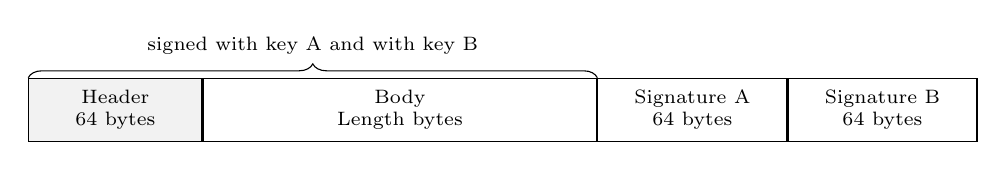
\begin{tikzpicture}[font=\scriptsize,
  seg/.style={draw, minimum height=0.8cm, align=center, inner sep=1pt}]
\node[seg, minimum width=2.2cm, fill=black!5] (h) at (0,0) {Header\\64 bytes};
\node[seg, minimum width=5.0cm, right=0pt of h] (b) {Body\\Length bytes};
\node[seg, minimum width=2.4cm, right=0pt of b] (a) {Signature A\\64 bytes};
\node[seg, minimum width=2.4cm, right=0pt of a] (s) {Signature B\\64 bytes};
\draw[decorate, decoration={brace, amplitude=5pt}] (h.north west) -- node[above=5pt]{signed with key A and with key B} (b.north east);
\end{tikzpicture}
\caption{A firmware image.}
\label{fig:image}
\end{figure}

\begin{figure}[H]
\centering
\begin{bytefield}[bitwidth=0.42cm]{32}
\bitbox[]{8}{\scriptsize byte 0} & \bitbox[]{8}{\scriptsize byte 1} & \bitbox[]{8}{\scriptsize byte 2} & \bitbox[]{8}{\scriptsize byte 3} \\
\wordbox{1}{Magic: the characters FSIR} \\
\bitbox{8}{Format} & \bitbox{8}{Kind} & \bitbox{16}{Target} \\
\wordbox{1}{Version} \\
\wordbox{1}{Length} \\
\wordbox{1}{Body check value} \\
\wordbox[lrt]{1}{Build identifier: 32 bytes} \\
\skippedwords \\
\wordbox[lrb]{1}{} \\
\wordbox{3}{Reserved: 12 bytes of 0x00} \\
\end{bytefield}
\caption{The image header. Kind: 0x01 bootloader, 0x02 main firmware, 0x03
last-resort firmware. Target: the controller identity [3,~REQ-046]. Body
check value: CRC-32 of the body, computed as for the frame. Build identifier: names the build that was
tested [3,~REQ-090].}
\label{fig:header}
\end{figure}

\begin{figure}[H]
\centering
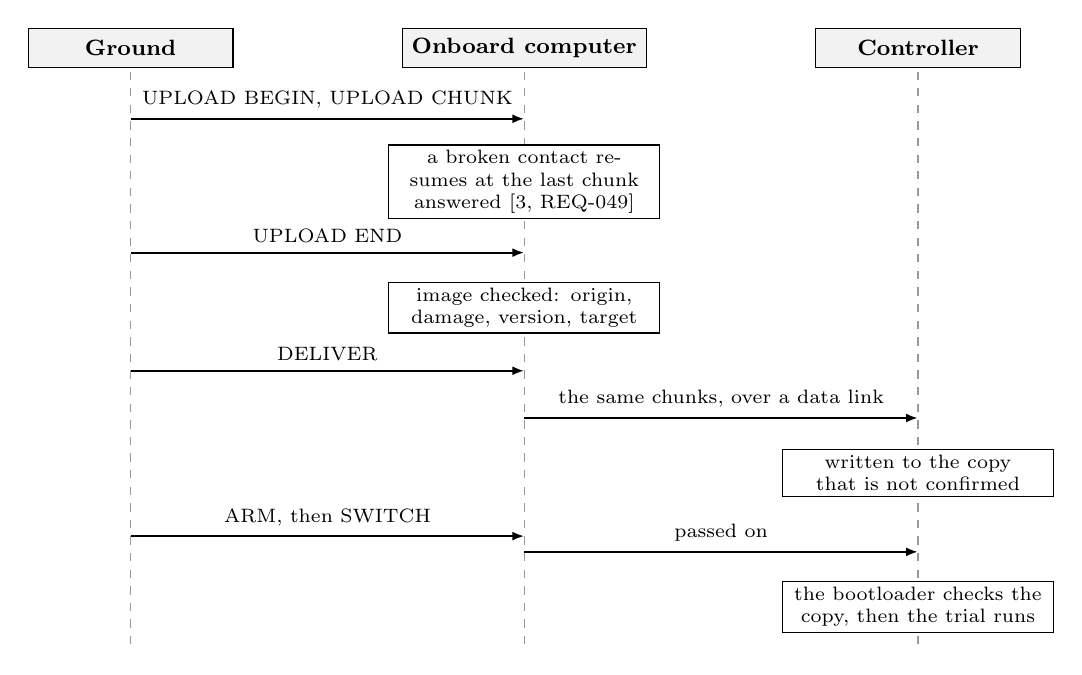
\begin{tikzpicture}[font=\scriptsize,
  head/.style={draw, fill=black!5, minimum width=2.6cm, minimum height=0.5cm, font=\footnotesize\bfseries},
  act/.style={draw, fill=white, text width=3.3cm, align=center, inner sep=2pt},
  msg/.style={-{Latex[length=1.5mm]}, thick}]
\node[head] at (0,0) {Ground};
\node[head] at (5,0) {Onboard computer};
\node[head] at (10,0) {Controller};
\foreach \x in {0,5,10} \draw[dashed, black!40] (\x,-0.3) -- (\x,-7.6);
\draw[msg] (0,-0.9) -- node[above]{UPLOAD BEGIN, UPLOAD CHUNK} (5,-0.9);
\node[act] at (5,-1.7) {a broken contact resumes at the last chunk answered \mbox{[3,~REQ-049]}};
\draw[msg] (0,-2.6) -- node[above]{UPLOAD END} (5,-2.6);
\node[act] at (5,-3.3) {image checked: origin, damage, version, target};
\draw[msg] (0,-4.1) -- node[above]{DELIVER} (5,-4.1);
\draw[msg] (5,-4.7) -- node[above]{the same chunks, over a data link} (10,-4.7);
\node[act] at (10,-5.4) {written to the copy that is not confirmed};
\draw[msg] (0,-6.2) -- node[above]{ARM, then SWITCH} (5,-6.2);
\draw[msg] (5,-6.4) -- node[above]{passed on} (10,-6.4);
\node[act] at (10,-7.1) {the bootloader checks the copy, then the trial runs};
\end{tikzpicture}
\caption{An update, as commands. Each command gets its two answers
(Figure~\ref{fig:answers}).}
\label{fig:update}
\end{figure}

% ===========================================================================
\section{Links}
The controller sits in a separate unit from the onboard computer, reached
through a cable harness. The links between the two units use balanced line
drivers, made for long distances and noisy environments [12,~Sec.~1, p.~3].

\subsection{Radio Link}
The radio equipment lies outside the System and is used as given
[5,~Sec.~1.2.2]. The ground software and the onboard computer software
exchange envelopes (Section~4.1) through it.

\subsection{Data Link A: UART over RS-422}
\label{sec:linka}
The UART runs at 115\,200 baud, 8 data bits, no parity, 1 stop bit; a frame
with a gap of more than 10\,ms inside it is dropped \tbr{uart}. Each direction
has its own RS-422 line, because an RS-422 line has one driver
[12,~Sec.~2, p.~3]. RS-422 sets no maximum cable length [12,~Sec.~2.1, p.~3].
On each data link the onboard computer sends GET STATUS every \tbd{beat}. A
link that misses \tbd{misses} answers in a row is reported lost [3,~REQ-081]
and is used again once it answers [3,~REQ-082].

\subsection{Data Link B: CAN}
\label{sec:linkb}
CAN is one of the interfaces that link units placed apart in a spacecraft
[13,~Sec.~8.2.2, p.~222]. Either end can start a transfer: a node sends once
the bus has been idle for a set time [14,~Sec.~3, p.~3], so the controller
sends its answers and reports without being asked. Each CAN frame carries its
own check value, and a frame received with an error is sent again
[14,~Sec.~3.1, p.~3]. Data link B uses CAN FD frames, which carry up to 64
data bytes [9,~Sec.~44.2, p.~1953], at a bit rate of \tbd{canrate}
\tbr{canfd}. A longer frame is split into segments
(Figure~\ref{fig:can}): each CAN frame carries a segment number in its first
byte, then up to 63 bytes of the frame. Segment 0 starts a frame; the receiver
joins the segments in order and checks the whole frame with its check value.
Each direction uses its own CAN identifier \tbr{canseg}.

\begin{figure}[H]
\centering
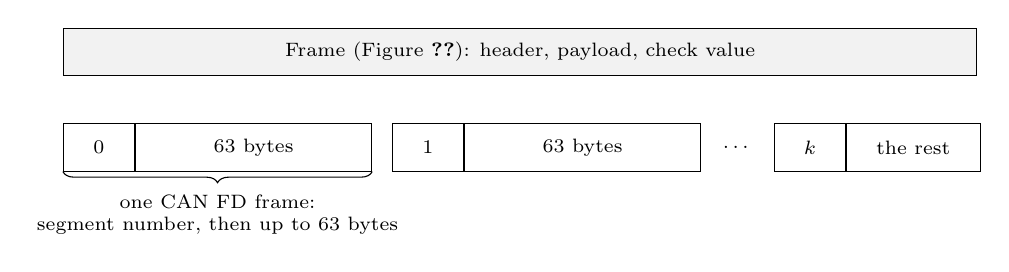
\begin{tikzpicture}[font=\scriptsize,
  seg/.style={draw, minimum height=0.6cm, align=center, inner sep=1pt}]
\node[seg, minimum width=11.6cm, fill=black!5] (f) at (0,0) {Frame (Figure~\ref{fig:frame}): header, payload, check value};
\node[seg, minimum width=0.9cm, anchor=north west] (n0) at ($(f.south west)+(0,-0.6)$) {0};
\node[seg, minimum width=3.0cm, right=0pt of n0] (d0) {63 bytes};
\node[seg, minimum width=0.9cm, right=0.25cm of d0] (n1) {1};
\node[seg, minimum width=3.0cm, right=0pt of n1] (d1) {63 bytes};
\node[right=0.15cm of d1] (dots) {\dots};
\node[seg, minimum width=0.9cm, right=0.15cm of dots] (nk) {$k$};
\node[seg, minimum width=1.7cm, right=0pt of nk] (dk) {the rest};
\draw[decorate, decoration={brace, amplitude=4pt, mirror}] (n0.south west) -- node[below=5pt, align=center]{one CAN FD frame:\\segment number, then up to 63 bytes} (d0.south east);
\end{tikzpicture}
\caption{A frame split into CAN FD frames.}
\label{fig:can}
\end{figure}

\subsection{Reprogramming Link A: SWD}
\label{sec:swd}
The onboard computer drives SWD from two general-purpose pins, with the
controller held stopped, so that no controller software runs
(Figure~\ref{fig:swd}).

\begin{figure}[H]
\centering
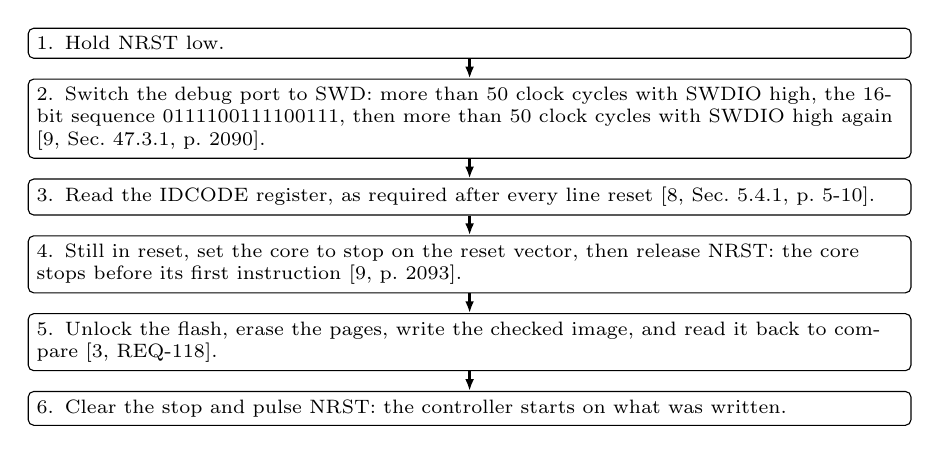
\begin{tikzpicture}[font=\scriptsize,
  st/.style={draw, rounded corners=2pt, text width=11cm, align=left, inner sep=3pt},
  ar/.style={-{Latex[length=1.5mm]}, thick}]
\node[st] (s1) at (0,0) {1. Hold NRST low.};
\node[st, below=0.25cm of s1] (s2) {2. Switch the debug port to SWD: more than 50 clock cycles with SWDIO high, the 16-bit sequence 0111100111100111, then more than 50 clock cycles with SWDIO high again [9,~Sec.~47.3.1, p.~2090].};
\node[st, below=0.25cm of s2] (s3) {3. Read the IDCODE register, as required after every line reset \mbox{[8,~Sec.~5.4.1, p.~5-10]}.};
\node[st, below=0.25cm of s3] (s4) {4. Still in reset, set the core to stop on the reset vector, then release NRST: the core stops before its first instruction [9,~p.~2093].};
\node[st, below=0.25cm of s4] (s5) {5. Unlock the flash, erase the pages, write the checked image, and read it back to compare [3,~REQ-118].};
\node[st, below=0.25cm of s5] (s6) {6. Clear the stop and pulse NRST: the controller starts on what was written.};
\foreach \a/\b in {s1/s2,s2/s3,s3/s4,s4/s5,s5/s6} \draw[ar] (\a) -- (\b);
\end{tikzpicture}
\caption{A restore through SWD.}
\label{fig:swd}
\end{figure}

\subsection{Reprogramming Link B: Factory Loader}
\label{sec:loader}
The factory loader's UART runs over its own RS-422 lines, as data link A does.
With the option bits as shipped (BOOT\_LOCK = 0, nBOOT1 = 1, nSWBOOT0 = 1), the
controller starts its factory loader when BOOT is high at reset
[11,~Table~2, p.~36]. The loader's protocol is fixed by its maker
(Figure~\ref{fig:loader}): 8 data bits, even parity, 1 stop bit
[11,~Table~115, p.~274]; the host sends 0x7F and the loader answers ACK, 0x79
[10,~p.~5]; every command byte is followed by its complement, every block
ends with the XOR of its bytes, and each packet is answered ACK 0x79 or NACK
0x1F [10,~p.~8].

\begin{figure}[H]
\centering
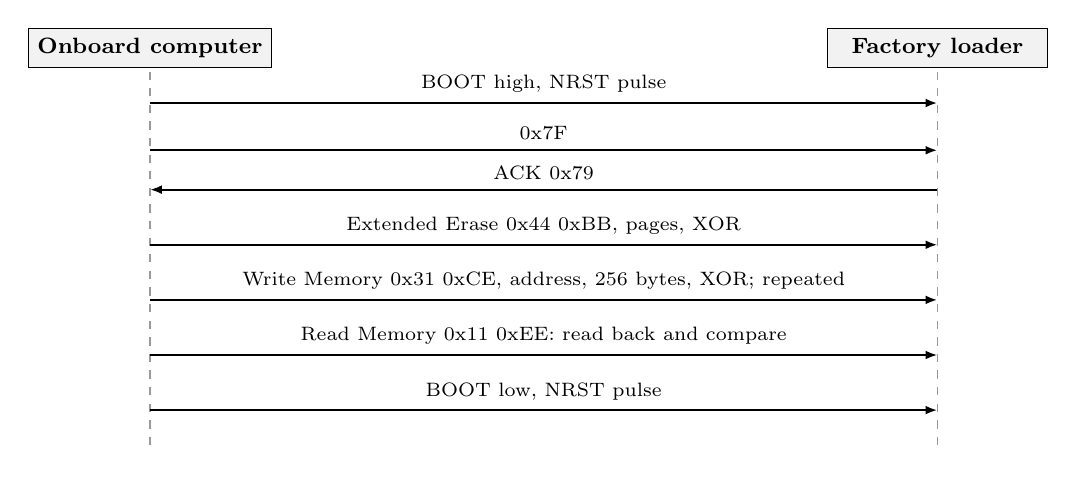
\begin{tikzpicture}[font=\scriptsize,
  head/.style={draw, fill=black!5, minimum width=2.8cm, minimum height=0.5cm, font=\footnotesize\bfseries},
  msg/.style={-{Latex[length=1.5mm]}, thick}]
\node[head] at (0,0) {Onboard computer};
\node[head] at (10,0) {Factory loader};
\foreach \x in {0,10} \draw[dashed, black!40] (\x,-0.3) -- (\x,-5.1);
\draw[msg] (0,-0.7) -- node[above]{BOOT high, NRST pulse} (10,-0.7);
\draw[msg] (0,-1.3) -- node[above]{0x7F} (10,-1.3);
\draw[msg] (10,-1.8) -- node[above]{ACK 0x79} (0,-1.8);
\draw[msg] (0,-2.5) -- node[above]{Extended Erase 0x44 0xBB, pages, XOR} (10,-2.5);
\draw[msg] (0,-3.2) -- node[above]{Write Memory 0x31 0xCE, address, 256 bytes, XOR; repeated} (10,-3.2);
\draw[msg] (0,-3.9) -- node[above]{Read Memory 0x11 0xEE: read back and compare} (10,-3.9);
\draw[msg] (0,-4.6) -- node[above]{BOOT low, NRST pulse} (10,-4.6);
\end{tikzpicture}
\caption{A restore through the factory loader. Each command is answered ACK
before the next one. Command codes from [10,~p.~7].}
\label{fig:loader}
\end{figure}

\noindent The onboard computer never sends the loader's Readout Protect
(0x82) or Write Protect (0x63) commands [10,~p.~7]: either would lock a way
back in [3,~REQ-125].

\subsection{Operator Interface}
The operator console shows every command with its state (sent, RECEIVED,
DONE or REFUSED with the reason), every command still waiting for an answer
[3,~REQ-094], which firmware runs [3,~REQ-095], and every report received. It
accepts commands, planned sequences of commands [3,~REQ-115] and firmware
releases. Signing with key~B needs the operator's hardware security key
[2,~Sec.~5.4].

% ===========================================================================
\section{Signals Between the Units}
The signals that cross the cable harness between the onboard computer and the
controller.

\smallskip
{\small\noindent\begin{tabularx}{\textwidth}{@{}l>{\raggedright\arraybackslash}Xll@{}}
\toprule
Signal & Interface & Direction & Electrical form \\
\midrule
UART line & data link A & TO CONTROLLER & RS-422 \\
UART line & data link A & TO ONBOARD COMPUTER & RS-422 \\
CANH, CANL & data link B & BOTH & CAN \\
SWDIO & reprogramming link A & BOTH & TBD \\
SWCLK & reprogramming link A & TO CONTROLLER & TBD \\
UART line & reprogramming link B & TO CONTROLLER & RS-422 \\
UART line & reprogramming link B & TO ONBOARD COMPUTER & RS-422 \\
NRST & reprogramming links A and B & TO CONTROLLER & TBD \\
BOOT & reprogramming link B & TO CONTROLLER & TBD \\
\bottomrule
\end{tabularx}}

\noindent{\small\textbf{Legend.} Direction: TO CONTROLLER, TO ONBOARD
COMPUTER, or BOTH. Electrical form: RS-422, one balanced line; CAN, the CAN
bus pair; TBD, not yet known \tbd{lines}.}

% ===========================================================================
\needspace{14\baselineskip}
\section{Safety Features}
Each feature of the interfaces that guards against a hazard of the hazard
analysis [4,~Sec.~4.0].

\smallskip
{\small\noindent\begin{tabularx}{\textwidth}{@{}>{\raggedright\arraybackslash}X>{\raggedright\arraybackslash}p{3.4cm}ll@{}}
\toprule
Feature & Interfaces & Hazards & Requirements \\
\midrule
Check value on every frame and image body & radio link, data links & H-7, H-9 & REQ-044, REQ-107 \\
Encryption and two signatures & radio link & H-2, H-5 & REQ-127 to 129 \\
Sequence numbers & radio link, data links & H-6 & REQ-031, REQ-065 \\
Expiry in every command & radio link, data links & H-6 & REQ-066, REQ-133 \\
Arming before a dangerous command & radio link, data links & H-6 & REQ-029, REQ-112 \\
Two answers to every command & radio link, data links & H-11 & REQ-033 \\
Failed envelopes dropped and logged & radio link & H-5 & REQ-064 \\
Link check on each data link & data links & H-4 & REQ-081 \\
CAN check value, and resend of a damaged CAN frame & data link B & H-7, H-9 & REQ-107 \\
Only checked images written & reprogramming links & H-2, H-7 & REQ-118 \\
No protection command sent to the loader & reprogramming link B & H-1 & REQ-125 \\
\bottomrule
\end{tabularx}}

% ===========================================================================
\appendix
\renewcommand{\thesection}{\Alph{section}}
\renewcommand{\thesubsection}{\Alph{section}.\arabic{subsection}}

\section{Acronyms}
\begin{description}[leftmargin=2.2cm]
\item[ACK] Acknowledge
\item[AES] Advanced Encryption Standard
\item[CAN] Controller Area Network
\item[CANH] CAN high line
\item[CANL] CAN low line
\item[CRC] Cyclic redundancy check
\item[GCM] Galois/Counter Mode
\item[NACK] Not acknowledge
\item[NRST] Reset pin
\item[SWCLK] SWD clock line
\item[SWD] Serial Wire Debug
\item[SWDIO] SWD data line
\item[TBD] To Be Determined
\item[TBR] To Be Resolved
\item[UART] Universal asynchronous receiver-transmitter
\end{description}

\section{Traceability}
Each requirement on an interface, and the section that meets it.

{\footnotesize
\begin{xltabular}{\textwidth}{@{}>{\raggedright\arraybackslash}X>{\raggedright\arraybackslash}p{5.2cm}@{}}
\toprule
Requirement & Section \\
\midrule
\endhead
REQ-064 to 066, REQ-107 & 4.0 Message Layer \\
REQ-127 to 129 & 4.1 Radio Envelope \\
REQ-027, REQ-028, REQ-031, REQ-033 to 035, REQ-100 & 4.2 Answers \\
REQ-019, REQ-021, REQ-053, REQ-055, REQ-058, REQ-073, REQ-074, REQ-084 to 086, REQ-113, REQ-117, REQ-121, REQ-132 & 5.1 Commands \\
REQ-029, REQ-030, REQ-112 & 5.2 Arming \\
REQ-068, REQ-069, REQ-134, REQ-136 & 5.3 Scheduled Commands \\
REQ-037 to 041, REQ-060, REQ-070 to 072, REQ-076, REQ-135 & 5.4 Reports \\
REQ-005, REQ-006, REQ-043 to 051, REQ-090 & 5.5 Firmware Images \\
REQ-080 to 082, REQ-138 & 6.2, 6.3 Data Links \\
REQ-083, REQ-118, REQ-122, REQ-125 & 6.4, 6.5 Reprogramming Links \\
REQ-094, REQ-095, REQ-115 & 6.6 Operator Interface \\
\bottomrule
\end{xltabular}}

\section{Open Items}
The values below are not yet known.
\begin{description}
\tbditem{ref}{Project name and document reference.}
\tbditem{equip}{Commands to the controlled equipment, the modes that accept
  them, and which are dangerous; the equipment is outside this project.}
\tbditem{arm}{Time after which an arming command expires [3, REQ-030].}
\tbditem{agree}{Largest allowed difference between the controller's clock and
  a scheduled run time [3, REQ-134].}
\tbditem{rate}{Rate of regular health reports [3, REQ-037].}
\tbditem{beat}{Interval of the link check on each data link.}
\tbditem{misses}{Number of missed answers in a row after which a data link is
  reported lost.}
\tbditem{canrate}{CAN bit rate of data link B.}
\tbditem{lines}{Electrical form of the SWD, NRST and BOOT lines between the
  units.}
\end{description}

\medskip
\noindent Section~4.0, and the Ed25519 signatures and AES-256 in Galois/Counter
Mode of Section~4.1, were accepted by the author on 12 October 2026. The
proposals below await the author's acceptance.
\begin{description}
\tbritem{priority}{Data link A and reprogramming link A used first; the B
  links used when the A links are lost (Section~3.0).}
\tbritem{silent}{A failed envelope gets no answer (Section~4.2).}
\tbritem{dangerous}{Which commands are dangerous (Section~5.1).}
\tbritem{armone}{An arming command allows one named command only
  (Section~5.2).}
\tbritem{sched}{A dangerous command cannot be scheduled (Section~5.3).}
\tbritem{uart}{The UART settings of data link A (Section~6.2).}
\tbritem{canfd}{CAN FD frames on data link B (Section~6.3).}
\tbritem{canseg}{The splitting of a frame into CAN frames, and one CAN
  identifier per direction (Section~6.3).}
\end{description}

\end{document}
